\documentclass[journal, twoside]{IEEEtran}
\IEEEoverridecommandlockouts
% The preceding line is only needed to identify funding in the first footnote. If that is unneeded, please comment it out.
\usepackage{cite}
\usepackage{amsmath,amssymb,amsfonts}
\usepackage{algorithmic}
\usepackage{graphicx}
\usepackage{textcomp}
\usepackage{xcolor}
\usepackage{stfloats}
\usepackage{multirow}
\usepackage{listings}
\usepackage{lipsum}
\usepackage{import}
% listing settings
\lstset{
  frame = lines,
  language = C,
  basicstyle = \ttfamily\footnotesize,
  breaklines = true,
}
% listing caption redefinition
\makeatletter
\def\lst@makecaption{%
  \def\@captype{table}%
  \@makecaption
}
\makeatother

\def\BibTeX{{\rm B\kern-.05em{\sc i\kern-.025em b}\kern-.08em
    T\kern-.1667em\lower.7ex\hbox{E}\kern-.125emX}}

\begin{document}

\bstctlcite{IEEEexample:BSTcontrol} % remove dashed repeated authors

\title{Investigating Performance Improvements\\in Discrete Space Hartree-Fock Calculations\\Through Graphics Processing Units\\{\large EECE542 Final Project Report}}
\author{\IEEEauthorblockN{Michel Kakulphimp}
\IEEEauthorblockA{\textit{Dept. of Electrical and Computer Engineering}\\
\textit{University of British Columbia}\\
Vancouver, Canada\\
michel@kakulphimp.net}
}

\markboth{UBC Winter 2021 EECE542: Nanoscale Modelling and Simulations}%
{}
\maketitle

\section{Introduction}

\section{Background and Related Work}

\subsection{Hartree-Fock Method}

The Hartree-Fock (HF) method \cite{szabo-ostlund} is designed to help approximate a solution to the Schr\"{o}dinger equation for many-electron systems. This is accomplished by making some key approximations, including: the Born-Oppenheimer approximation to fix the kinematics of the nucleus, using a single Slater determinant composed of orthogonal molecular spin orbitals to satisfy the Pauli exclusion principle, and most importantly approximating the Hamiltonian as a single electron function by treating the other electrons in the system as a mean field rather than evaluating with their exact states. HF iteratively converges to its solution by progressively making better guesses at the structure of the mean field of the system. Combined, these techniques help reduce the original multivariate and computationally intensive problem into one that is easily solved by a computer program. One such implementation is described within this report, where we perform the restricted, closed-shell HF algorithm on a Helium atom.

Since Helium has an even number of electrons that close shells, we can use the restricted HF (RHF) equation for closed shell systems to numerically calculate the resulting orbitals. The equation is as follows:

\begin{align}
  \hat{F}(\vec{r})\psi_n(\vec{r}) &= \epsilon_n\psi_n(\vec{r})
\end{align}

Where $\hat{F}(\vec{r})$ is the Fock operator which is defined as follows:

\begin{align}
  \hat{F}(\vec{r}) &= \hat{H}_{core}(\vec{r}) + \sum_{n=1}^{N/2}\left[2J_n(\vec{r}) - K_n(\vec{r})\right]
\end{align}

The Fock operator is composed of the core Hamiltonian operator $\hat{H}(\vec{r})$, the Coulomb operator $\hat{J}(\vec{r})$, and the exchange operator $\hat{K}(\vec{r})$.

\begin{align}
  \hat{H}_{core}(\vec{r}) &= -\frac{1}{2}\nabla_1^2 - \sum_A\frac{Z_A}{\|\vec{r}_{1 A}\|}\\
  \hat{J}_j(\vec{r}_1)\psi_i(\vec{r}_1) &= \psi_i(\vec{r}_1)\int_{-\infty}^{\infty}\left|\psi_i(\vec{r}_2)\right|^2\frac{1}{\|\vec{r}_{12}\|}d\vec{r}_2 \\
  \hat{K}_j(\vec{r}_1)\psi_i(\vec{r}_1) &= \psi_j(\vec{r}_1)\int_{-\infty}^{\infty}\frac{\psi_j^\ast(\vec{r}_2)\psi_i(\vec{r}_2)}{\|\vec{r}_{12}\|}d\vec{r}_2
\end{align}

By discretizing the solution space of the problem into $N$ partitions in the three Cartesian coordinate directions and representing the Fock equation in matrix form, we can solve for the discretized wave equation $\psi_n(\vec{r})$ by solving for the eigenvectors of the Fock matrix. For each iteration of the HF algorithm, a new guess is obtained for the discretized wave equation, which can be used to compute the Fock matrix for the following iteration. If initial conditions are favorable, the iterations will eventually settle on a solution with little to no variation. The numeric value of the total energy of the system on every iteration can be used as an indicator for convergence.

This report does not take the concept of HF further than what is presented; however, it is important to note that there is are numerous improvement on the technique. One such improvement uses the Roothaan-Hall equations, by representing the solution wave functions through a linear combination of known spatial basis equations. This allows HF to take another matrix form and has the benefit of being much lighter in terms of computation. Since the techniques discussed in the report target fundamental computations shared by HF and its derivatives, they can of course be applied to them as well.

\subsection{CUDA Parallel Computing Platform}

Graphics processing units (GPUs) are primarily designed to accelerate the computational requirements of real-time raster 3D graphics. However, their hardware is also well suited for accelerating other, highly parallelizable workloads. This is made possible by GPU manufacturers providing APIs that allow developers to write specially designed software to run on the CPUs. Since GPUs have a fundamentally different architecture than CPUs, the software must be written with the architecture in mind and must also be compiled as a separate executable entity to be run exclusively on the GPU. In an example implementation of GPU acceleration, a developer identifies workloads that are well suited for the architecture of a GPU to accelerate and write routines to be executed exclusively on the GPU. The host program would then call these routines and provide the necessary data for the GPU to perform execution and return results.

NVIDIA, a GPU manufacturer, provides one such API for developers called Computer Unified Architecture or CUDA. It is also known as the CUDA parallel computing platform \cite{nvidia-cuda}. As an NVIDIA-based GPU

% What CUDA provides
% GPU architecture
% GPU limitations
% CPU-GPU memory transfers

\cite{nvidia-cuda}

\section{Acceleration Opporunities}

\subsection{Numerical Integration}

\subsection{Eigensolver}

\section{Implementation}

For this investigation, a program written in C++ was created to evaluate the acceleration of the eigensolver and the numerical integration on a discrete space HF solver for the Helium atom. The program is designed to be able to variably define the number of partitions used in the discretization of the solution space and selectively run the eigensolver and numerical integration on either the CPU or the GPU. C++ was chosen as the programming language as it is straightforward to integrate with the CUDA C APIs and the language has wide support in terms of libraries for utilities. To facilitate the linear algebra operations required by HF, the Eigen \cite{eigen} C++ template library was chosen. This provides structures and types to support matrix arithmetic. Eigen was linked with AMD Basic Linear Algebra Subprograms (BLAS) libraries \cite{amd-blas} to provide low level multi-core CPU support for matrix operations. Eigen was also linked with LAPACK (Linear Algebra PACKage) \cite{lapack} libraries which are used in higher-level linear algebra operations such as those to compute the eigenvectors and eigenvalues of a matrix. OpenMP is used to enable multiprocessor support for the CPU BLAS and LAPACK operations, and the LAPACKE C API is used to wrap around the LAPACK libraries which are written in Fortran. Finally, the C++ Boost libraries provide the program with quality of life tools for things such as command line arguments parsing and string formatting.

Due to the locality requirements of the data to be computed on, the program is architected in such a way where GPU accelerated routine data can either be allocated in RAM or in VRAM. In a CPU-only run of a routine, the data is only allocated on the CPU side and remains resident in RAM. However, in the GPU-accelerated run of a routine, data required for computation is allocated and copied over to the GPU's VRAM over PCIe. Once GPU computation is complete, the resulting data is copied back to the host RAM. The Eigen template library provides a means to map its matrix and vector structures over a pointer to data in memory, allowing for this dynamically allocated data to be computed on during matrix arithmetic.

% List features of the program, how it's structured (the cfg/lut for example), and how at runtime the CPU or the GPU is chosen
% Add any other details relating to the implementation of the program

\section{Results}

The results for this investigation were obtained using a personal computing platform with the following relevant technical specifications:

\begin{itemize}
    \item CPU: AMD Ryzen 9 5950X 16-Core Processor
    \item RAM: 64 GB DDR4
    \item GPU: NVIDIA GeForce RTX 3080 Ti
    \item VRAM: 12 GB GDDR6X
    \item CPU-GPU Interconnect: PCIe 4.0 x16 (32 GB/s maximum bandwidth)
\end{itemize}

\begin{figure*}[ht]
\centering
\includegraphics[width=7in]{figures/one-core-results.pdf}
\caption{Performance Results Per Iteration (1 CPU Thread)}
\label{perf-results-per-iteration-one-core}
\end{figure*}

\begin{figure*}[ht]
\centering
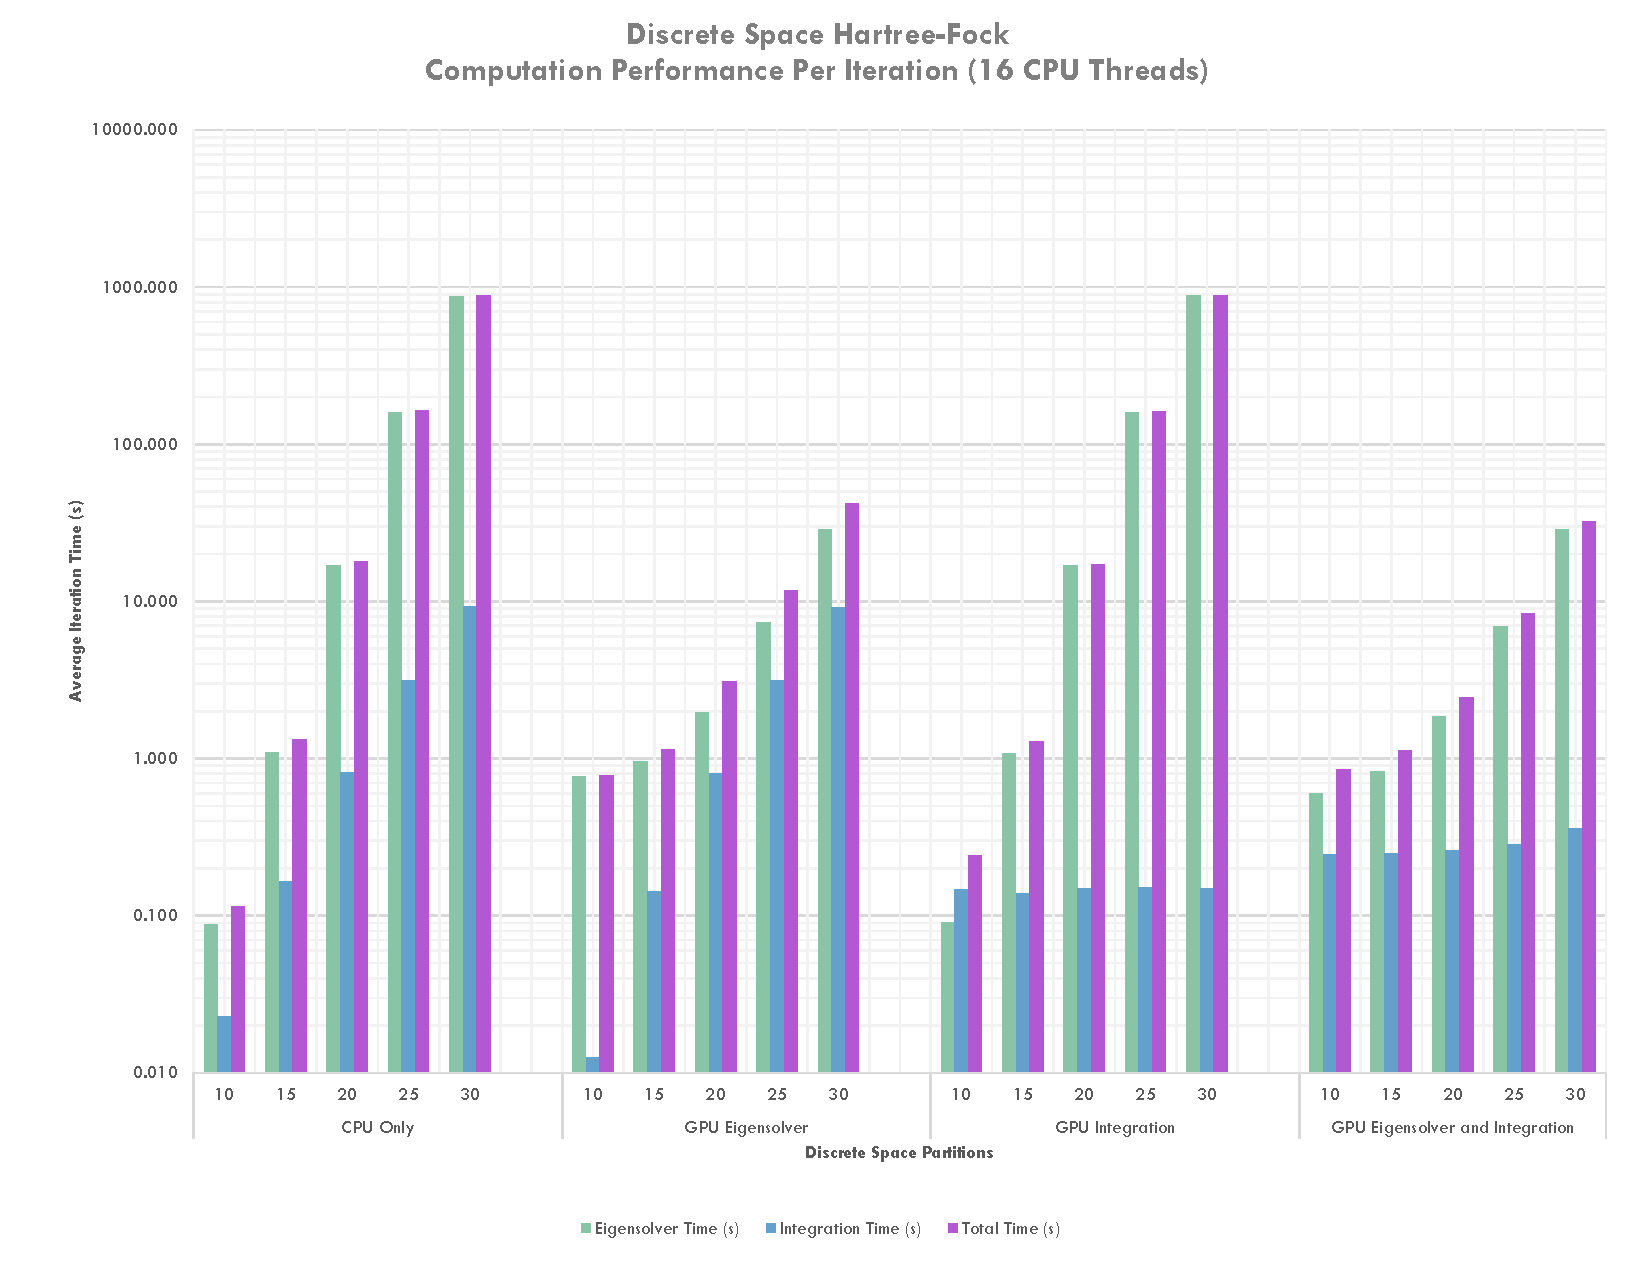
\includegraphics[width=7in]{figures/sixteen-core-results.pdf}
\caption{Performance Results Per Iteration (16 CPU Threads)}
\label{perf-results-per-iteration-sixteen-core}
\end{figure*}

% Mention overhead that show up in results when integrating on GPU

\begin{table*}
    \renewcommand{\arraystretch}{1.3} % vertically stretch table out
    \caption{5 MB Workload Execution Times (1 millisecond dead-time)}
    \label{main-workload-results-1ms}
    \centering
    \begin{tabular}{c||c|c|c|c|c|c|c|c}
        \hline
        \multirow{2}{*}{Scaling Policy} & \multicolumn{8}{c}{Power-Loss Profile Period Sweep (Sawtooth-Down) Runtimes (s)} \\\cline{2-9}
        {} & {10 ms to 8 ms} & {S.F.} & {10 ms to 4 ms} & {S.F.} & {10 ms to 2 ms} & {S.F.} & {10 ms to 1 ms} & {S.F.} \\
        \hline
        \hline
        {Baseline}                  & {48.429} & {1.00} & {48.429}  & {1.00} & {48.429}  & {1.00} & {48.429}  & {1.00}\\
        {Linear Scaling}            & {86.326} & {1.78} & {85.405}  & {1.76} & {153.755} & {3.18} & {462.042} & {9.54}\\
        {Random Adaptive Scaling}   & {95.498} & {1.97} & {117.985} & {2.44} & {119.484} & {2.47} & {132.488} & {2.74}\\
        {Linear Adaptive Scaling}   & {95.611} & {1.97} & {94.244}  & {1.95} & {110.304} & {2.28} & {124.021} & {2.56}\\
        \hline
    \end{tabular}
\end{table*}

\begin{table*}
    \renewcommand{\arraystretch}{1.3} % vertically stretch table out
    \caption{5 MB Workload Execution Times (500 microsecond dead-time)}
    \label{main-workload-results-500us}
    \centering
    \begin{tabular}{c||c|c|c|c|c|c|c|c}
        \hline
        \multirow{2}{*}{Scaling Policy} & \multicolumn{8}{c}{Power-Loss Profile Period Sweep (Sawtooth-Down) Runtimes (s)} \\\cline{2-9}
        {} & {10 ms to 8 ms} & {S.F.} & {10 ms to 4 ms} & {S.F.} & {10 ms to 2 ms} & {S.F.} & {10 ms to 1 ms} & {S.F.} \\
        \hline
        \hline
        {Baseline}                  & {45.811} & {1.00} & {45.811}  & {1.00} & {45.811} & {1.00}  & {45.811}  & {1.00}\\
        {Linear Scaling}            & {71.445} & {1.56} & {69.302}  & {1.51} & {80.453} & {1.76}  & {255.806} & {5.58}\\
        {Random Adaptive Scaling}   & {75.260} & {1.64} & {79.272}  & {1.73} & {86.970} & {1.90}  & {95.449}  & {2.08}\\
        {Linear Adaptive Scaling}   & {65.013} & {1.42} & {74.533}  & {1.63} & {82.870} & {1.81}  & {87.939}  & {1.92}\\
        \hline
    \end{tabular}
\end{table*}

\begin{table*}
    \renewcommand{\arraystretch}{1.3} % vertically stretch table out
    \caption{Workload Execution Times (1000 microsecond dead-time)}
    \label{workload-size-performance}
    \centering
    \begin{tabular}{c||c|c|c|c|c}
        \hline
        \multirow{2}{*}{Scaling Policy} & \multicolumn{4}{c|}{Workload Runtimes (s)}\\\cline{2-6}
        {} & {5 MB} & {4 MB} & {2 MB} & {1 MB} & {R\textsuperscript{2}}\\
        \hline
        \hline
        {Baseline}                  &  {48.429} &  {38.749} &  {19.373} &   {9.688} & {1.0}\\
        {Linear Scaling}            & {462.042} & {359.176} & {154.856} &  {52.047} & {1.0}\\
        {Linear Adaptive Scaling}   & {124.021} &  {97.080} &  {47.392} &  {23.261} & {1.0}\\
        \hline
    \end{tabular}
\end{table*}

\begin{table*}
    \renewcommand{\arraystretch}{1.3} % vertically stretch table out
    \caption{5 MB Workload Execution Times (1 millisecond dead-time)}
    \label{power-loss-profile-performance}
    \centering
    \begin{tabular}{c||c|c|c|c}
        \hline
        \multirow{2}{*}{Scaling Policy} & \multicolumn{4}{c}{Power-Loss Profile (10 ms to 1 ms Sweep) Runtimes (s)} \\\cline{2-5}
        {} & {Sawtooth-Down} & {Sawtooth-Up} & {Sine} & {Square}\\
        \hline
        \hline
        {Baseline}                  &  {48.429} &  {48.429} &  {48.429} &  {48.429}\\
        {Linear Scaling}            & {462.042} & {512.373} & {523.763} & {885.978}\\
        {Linear Adaptive Scaling}   & {124.021} & {123.280} & {123.580} & {173.061}\\
        \hline
    \end{tabular}
\end{table*}

\section{Future Work}

\section{Conclusion}

\bibliographystyle{IEEEtran}
\bibliography{IEEEabrv, refs}

\end{document}